\section{问题重述}
\label{sec:problem}

\subsection{问题背景}
\subsubsection{资源要素与标度律}
大语言模型（large language model, LLM）的训练可看作在有限算力下对若干资源要素的联合配置：
参数量 $N$ 决定模型容量，训练 token 数 $D$ 决定数据规模，总算力 $C$ 决定可支付的训练成本，
数据质量 $Q$ 刻画语料的可用程度，领域配比 $\boldsymbol{p}$ 则决定算力在各训练领域之间的分配。
经典标度律（scaling law）以幂律形式描述验证集交叉熵损失 $L$ 随 $N$、$D$ 的变化，
其常见形式为
\begin{equation}
  L(N,D)=E+A\,N^{-\alpha}+B\,D^{-\beta},
  \label{eq:classic-law}
\end{equation}
其中 $E$ 为不可约损失，$A,\alpha,B,\beta$ 为待估参数\citep{kaplan2020,hoffmann2022}。
\eqref{eq:classic-law}并不显式包含数据质量与领域配比，而这两者恰恰是当前语料工程的主要着力点。

\subsubsection{数据墙与数据质量}
高质量语料的增长远慢于算力与模型规模的扩张，可用干净数据的稀缺已构成所谓数据墙（data wall）
问题，在数据受限条件下继续扩大训练量的收益会显著衰减\citep{muennighoff2023}。
与此同时，数据筛选与质量治理的收益被反复观察到：以检索增强方式构造科学文献问答的小规模模型，
可以在部分任务上超过参数量高出一个量级以上的通用模型\citep{asai2026openscholar}；
而在固定算力预算下，数据筛选策略本身也服从标度关系，筛选比例并非越高越好\citep{goyal2024filtering}。
这提示在算力受限时，把预算投向数据质量而非单纯堆叠参数量或 token 数，可能获得更高的边际收益。

\subsubsection{上下文长度与配比的成本}
扩大规模、提升质量与延长上下文长度都需要付出算力代价，三者相互挤占。
长文本带来的注意力计算与 KV 缓存开销随上下文长度线性增长，构成一项与 $N$、$D$ 同时相关的额外成本；
而调整领域配比本身不增加总算力，但会改变算力在各领域间的分配效果。
围绕数据配比已有若干可操作的经验规律：配比可用回归方法在较小规模上预测\citep{liu2024regmix}，
领域权重可在训练过程中动态优化\citep{xie2023doremi}，领域与技能之间的结构性差异也会改变最优配比
\citep{chen2023skillit}，而数据选择方法的整体图景见\citet{albalak2024survey}。
本赛题要求以公开数据与已标注可信度的半合成数据为据，建立 $N$、$D$、$Q$、$\boldsymbol{p}$ 与 $L$ 的关系，
并在此基础上研究算力约束下的资源配置。

\subsection{数据条件}
\label{subsec:data}
赛题附件共 40 个文件、约 551\,MB，按所服务的问题分为三组（附件编号与文件名的对照见《数据说明》）。
图~\ref{fig:data-pipeline}给出数据的整体构成与本队的处理路径。

\begin{figure}[htbp]
  \centering
  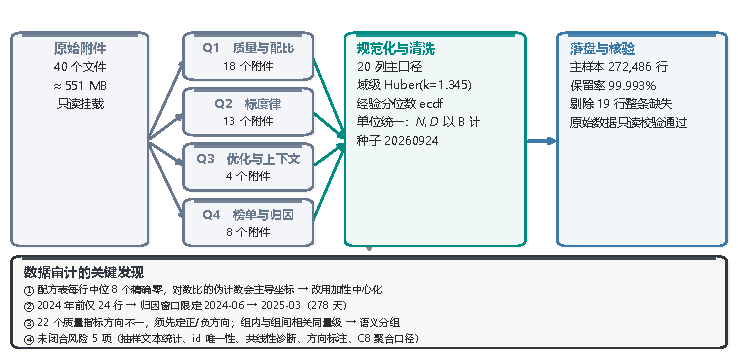
\includegraphics[width=0.98\linewidth]{figures/fig_data_pipeline.pdf}
  \caption{附件数据的构成、按问映射与规范化流程。左侧为 40 个原始附件（只读），
  中部为按子问题划分的输入集，右侧为规范化、清洗与一致性核验环节。}
  \label{fig:data-pipeline}
\end{figure}

\textbf{附件 A（质量信号与配方实验）}服务问题一。其中 A1 为质量主样本（51\,230 条 $\times$ 27 字段），
A2、A3 为 arxiv 与 github 两个域的扩展集（17\,523 条与 203\,752 条），三者合为 22 个质量指标的
全量记录；A4--A11 为 1M、60M、1B 三个尺度下的训练与检验配方及其对应 Loss；
A12--A15 为 10B、70B 的外推表，其配比取自训练集子集、Loss 由三尺度幂律外推；
A16 为质量域与配方域之间的人工映射参考，A18 为对原文抽样得到的文本统计量。

\textbf{附件 B（标度律轨迹）}服务问题二。B1、B3 为 Pythia 真实训练轨迹\citep{biderman2023pythia}，
B2 为经真实数据校准并注入噪声的半合成轨迹，B4 为跨模型族收敛点，B5 为文献标度律数值；
B6--B8 为基于真实数据校准的半合成因子设计网格，是附件中唯一含数据质量因子的部分；
B9、B10 给出百亿参数以上的报告值与外推值，用于讨论外推可信度边界。

\textbf{附件 C（评测榜单）}服务问题四。C1 为 Open LLM Leaderboard 的投榜记录\citep{beeching2023leaderboard}，
C3 为其时间序列版本，C4 为模型元数据（含参数量与开源权重字段），C5、C6 为 Loss 与榜分的桥接数据，
C7 为架构元数据并给出上下文长度的可行取值，C8 为 BBH 等基准的逐任务评测明细。

按题目要求的可信度分级，A4--A11、B1、B4、B5、C1--C4、C8 等属真实观测；A12--A15、A13、A15
与 B10 为外推或子集；B2、B6、B7、B8 为半合成数据。后两类在后续各节首次使用时均标明其性质，
其结论仅作补充分析，不作为直接实验观测。

\subsection{任务说明}
赛题四问构成一条递进主线，前一问的输出是后一问的输入。

\textbf{问题一}要求在统一 22 个质量指标方向的前提下建立综合评价模型，给出样本级、语料级或领域级的
质量评分 $Q$；定义并分析指标之间的冲突，给出消解规则；并利用配方实验数据建立 17 域配比
$\boldsymbol{p}$（满足单纯形约束）与交叉熵损失之间的定量关系，同时在检验集上验证、在外推表上讨论稳健性。
是否以及如何把质量评分引入配比模型，由本队论证。

\textbf{问题二}要求综合问题一输出的 $Q$ 与 $\boldsymbol{p}$，建立同时包含 $N$、$D$、$Q$、$\boldsymbol{p}$
的广义标度律，说明其相对经典形式的退化行为，分析各因素的边际效用与弹性，讨论领域之间的替代或互补关系，
并推导提升数据质量与扩大模型规模可相互替代的条件。

\textbf{问题三}要求在总算力预算 $C$ 的约束下求解 $N$、$D$、$Q$、$\boldsymbol{p}$ 的最优配置。
算力消耗由基础训练开销 $C_{\text{train}}=6ND$、质量提升开销
$C_{Q}=D\,[g(Q)-g(Q_{0})]_{+}$ 与长文本注意力开销 $C_{\text{attn}}=\eta N D L_{\text{ctx}}$
三部分构成，其中 $\eta=2\times10^{-4}$，$L_{\text{ctx}}$ 由架构与任务需求外生给定。
本问还要求讨论成本函数 $g$ 的选取对最优解的影响，并分析预算跨越不同量级时资源分配是否发生结构性转移，
且须给出该转移的数学定义与识别方法。

\textbf{问题四}要求利用评测榜单数据分离并量化规模扩张与非规模技术进步对模型能力的贡献，
在算力增长放缓的情景下预测未来 12 个月或 24 个月开源模型的能力前沿并给出不确定性分析；
还要求建立交叉熵损失与多维基准得分之间的映射，并讨论映射误差对结论的影响。

四个子问题共享同一套数据与参数体系：问题一的 $Q$ 与 $\boldsymbol{p}$ 进入问题二，
问题二的标度律参数进入问题三与问题四的预测环节，问题三的优化结果又反过来解释问题四所观察到的规模变化。
本文的整体框架与证据链见图~\ref{fig:framework-overall}。
